% 去掉`titlepage`后不生成封面
\documentclass[titlepage,openany]{SHUugt}

\usepackage{graphicx}
\usepackage{verbatim}
\usepackage{listings}
\usepackage{multirow}
\usepackage{longtable}
\usepackage{float}
\usepackage{booktabs}

\begin{document}

% 课题和作者
\title{你的大作}
\author{你的名字}
\college{你的学院}
\department{你的专业}
\stunumber{你的学号}
\teacher{你的指导教师}

% 这里用*LaTeX*写你的中文概要
\cabstract{

这里是你的\emph{中文}概要。

}
% 你的中文关键字
\ckeywords{关键字1, 关键字2, 关键字3, Keyword4}

% 这里用*LaTeX*写你的英文概要
\eabstract{

This is your \emph{English} abstract.

}
% 你的英文关键字
\ekeywords{Keyword1, Keyword2, Keyword3, Keyword4}


\makecover

\chapter{绪言}\label{ux7eeaux8a00}

使用\href{http://johnmacfarlane.net/pandoc/README.html}{Pandoc
Markdown}写论文的正文。

阅读\texttt{thesis.md}、\texttt{template.tex}、\texttt{abstract.tex}、\texttt{thanks.md}来看看这篇文章是从什么样的源码生成的。

\chapter{章节1}\label{ux7ae0ux82821}

\section{引用}\label{ux5f15ux7528}

请在\texttt{ref.bib}里添加引用文献,然后可以这样引用\cite{aumann1976agreeing},也可以让标号出现在右上角\citeu{aumann1976agreeing}。

\texttt{ref.bib}中所有的条目都出现在参考文献一节中,而不仅仅是被引用的条目。

\section{列表}\label{ux5217ux8868}

\subsection{无序列表}\label{ux65e0ux5e8fux5217ux8868}

\begin{itemize}
\tightlist
\item
  here is my first list item.
\item
  and my second.
\end{itemize}

\subsection{有序列表}\label{ux6709ux5e8fux5217ux8868}

\begin{enumerate}
\def\labelenumi{\arabic{enumi}.}
\tightlist
\item
  one
\item
  two
\item
  three
\end{enumerate}

\section{代码}\label{ux4ee3ux7801}

\subsection{行内代码}\label{ux884cux5185ux4ee3ux7801}

这是行内代码\texttt{print\ 1\ +\ 1}。

\subsection{代码片段}\label{ux4ee3ux7801ux7247ux6bb5}

\begin{verbatim}
qsort []     = []
qsort (x:xs) = qsort (filter (< x) xs) ++ [x] ++
               qsort (filter (>= x) xs)
\end{verbatim}

\section{表格}\label{ux8868ux683c}

\begin{longtable}[]{@{}rlcl@{}}
\caption{Demonstration of simple table
syntax\label{table:simple}.}\tabularnewline
\toprule
Right & Left & Center & Default\tabularnewline
\midrule
\endfirsthead
\toprule
Right & Left & Center & Default\tabularnewline
\midrule
\endhead
12 & 12 & 12 & 12\tabularnewline
123 & 123 & 123 & 123\tabularnewline
1 & 1 & 1 & 1\tabularnewline
\bottomrule
\end{longtable}

\section{图}\label{ux56fe}

图请放入\texttt{figures}目录下。

\begin{figure}
\centering
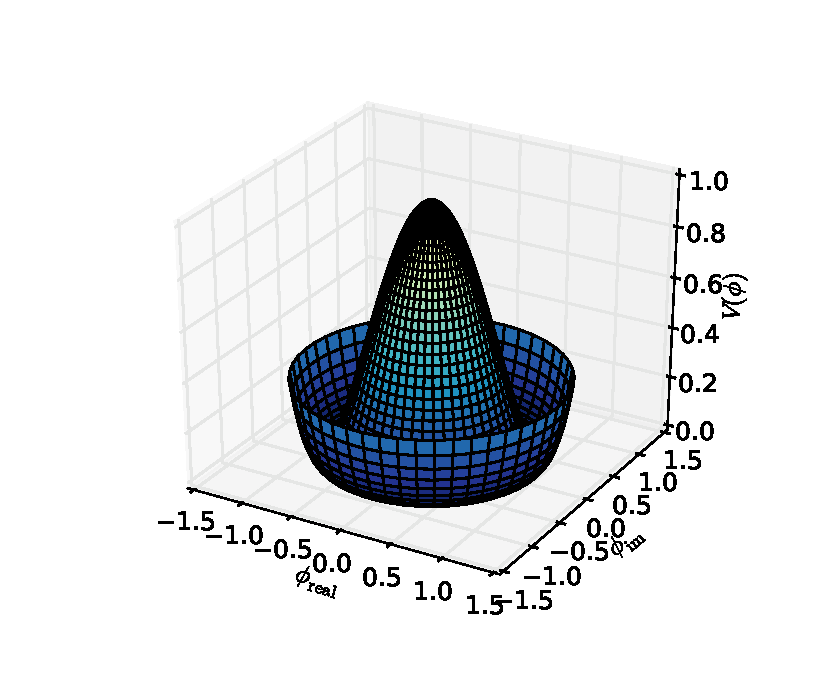
\includegraphics{figures/radial.pdf}
\caption{图示例\label{fig:radial}}
\end{figure}

\section{公式}\label{ux516cux5f0f}

\subsection{行内公式}\label{ux884cux5185ux516cux5f0f}

这是行内公式\(\sum_{i=1}^{10} t_i\)。

\subsection{块公式}\label{ux5757ux516cux5f0f}

\begin{equation}
  x = a_0 + \cfrac{1}{a_1
          + \cfrac{1}{a_2
          + \cfrac{1}{a_3 + \cfrac{1}{a_4} } } }
\end{equation}

\begin{equation}
  \lim_{x \to \infty} \exp(-x) = 0
\end{equation}

\section{交叉引用}\label{ux4ea4ux53c9ux5f15ux7528}

\begin{enumerate}
\def\labelenumi{\arabic{enumi}.}
\tightlist
\item
  如表格\ref{table:simple}所示;
\item
  如图\ref{fig:radial}所示。
\end{enumerate}

\chapter{章节2}\label{ux7ae0ux82822}

可以自定义LaTeX指令。

\newcommand{\ugt}{This is a command named \texttt{{\textbackslash}ugt}}

\ugt

\addcontentsline{toc}{chapter}{致\hspace{1.5em}谢}
\chapter*{致\hspace{2em}谢}
这里是用Markdown写的\emph{致谢}。

由于本人学识有限,加之时间仓促,文中不免有错误和待改进之处,真诚欢迎各
位师长、同行提出宝贵的意见。


\backmatter
\nocite{*}
\bibliographystyle{shu}
\bibliography{ref}

\end{document}
